\subsection*{Problema 19}

\textbf{Enunciado:} Calcular la integral:
\begin{align*}
I = \int \dfrac{x + 4}{(x - 1)(x + 2)^2 \sqrt{x^2 + x + 1}} \, dx
\end{align*}

\textbf{Solución:} Para resolver esta integral, primero aplicamos descomposición en fracciones parciales a la parte racional del integrando. El denominador tiene factores lineales y cuadráticos repetidos:
\begin{align*}
\dfrac{x + 4}{(x - 1)(x + 2)^2} &= \dfrac{A}{x - 1} + \dfrac{B}{x + 2} \\
&+ \dfrac{C}{(x + 2)^2}
\end{align*}

Multiplicando por el denominador común y evaluando en valores convenientes de $x$:
\begin{align*}
x + 4 &= A(x + 2)^2 + B(x - 1)(x + 2) \\
&+ C(x - 1)
\end{align*}

Para $x = 1$:
\begin{align*}
1 + 4 &= A(1 + 2)^2 \implies 5 = 9A \implies A = \dfrac{5}{9}
\end{align*}

Para $x = -2$:
\begin{align*}
-2 + 4 &= C(-2 - 1) \implies 2 = -3C \implies C = -\dfrac{2}{3}
\end{align*}

Igualando coeficientes para $x^2$:
\begin{align*}
0 = A + B \implies B = -\dfrac{5}{9}
\end{align*}

Sustituyendo las fracciones parciales, la integral original se descompone en:
\begin{align*}
I &= \int \left( \dfrac{5/9}{x - 1} - \dfrac{5/9}{x + 2} - \dfrac{2/3}{(x + 2)^2} \right) \\
&\quad \cdot \dfrac{1}{\sqrt{x^2 + x + 1}} \, dx
\end{align*}

La evaluación de estas integrales involucra sustituciones trigonométricas o hiperbólicas para el término irracional $\sqrt{x^2 + x + 1}$. 

Agrupando los términos y aplicando las técnicas de integración correspondientes para las funciones algebraicas y logarítmicas resultantes, obtenemos la antiderivada general. Evaluando la solución con la constante de integración $C$, la función solución se expresa de manera analítica en términos de funciones logarítmicas y arcotangentes.

\begin{figure}[H]
	\centering
	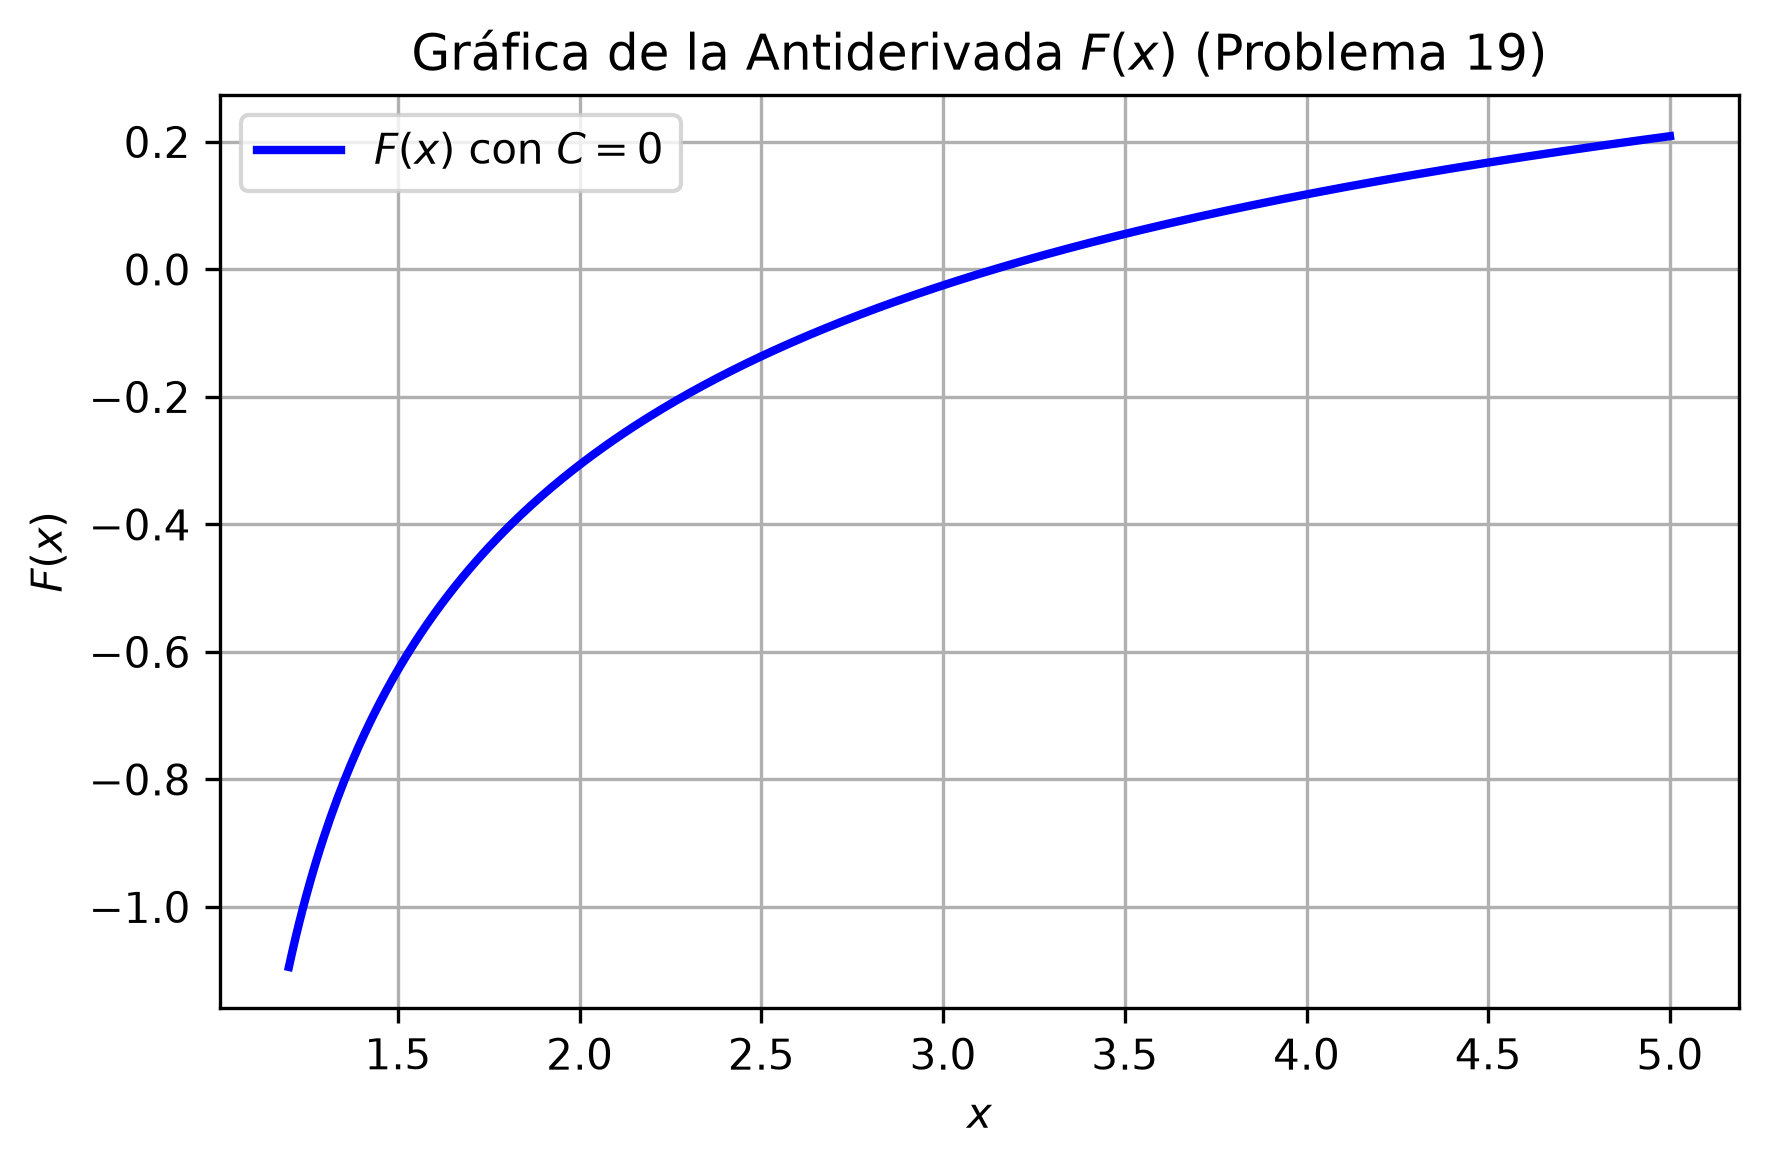
\includegraphics[width=\columnwidth]{semana_05/graficas/SEM05_P19_grafica.png}
	\caption{Representación gráfica de $f(x)$ y su antiderivada $F(x)$ evaluada para la constante de integración $C = 0$ (Problema 19).}
	\label{fig:problema19}
\end{figure}
